\documentclass{article}
\usepackage{amsmath}
\usepackage{color,pxfonts,fix-cm}
\usepackage{latexsym}
\usepackage[mathletters]{ucs}
\DeclareUnicodeCharacter{8211}{\textendash}
\DeclareUnicodeCharacter{8220}{\textquotedblleft}
\DeclareUnicodeCharacter{46}{\textperiodcentered}
\DeclareUnicodeCharacter{8221}{\textquotedblright}
\DeclareUnicodeCharacter{60}{\textless}
\DeclareUnicodeCharacter{62}{\textgreater}
\DeclareUnicodeCharacter{183}{$\cdot$}
\DeclareUnicodeCharacter{32}{$\ $}
\usepackage[T1]{fontenc}
\usepackage[utf8x]{inputenc}
\usepackage{pict2e}
\usepackage{wasysym}
\usepackage[english]{babel}
\usepackage{tikz}
\pagestyle{empty}
\usepackage[margin=0in,paperwidth=612pt,paperheight=792pt]{geometry}
\begin{document}
\definecolor{color_29791}{rgb}{0,0,0}
\begin{tikzpicture}[overlay]\path(0pt,0pt);\end{tikzpicture}
\begin{picture}(-5,0)(2.5,0)
\put(500.14,-731.336){\fontsize{12}{1}\usefont{T1}{cmr}{m}{n}\selectfont\color{color_29791}1 }
\put(60.024,-730.616){\fontsize{9.96}{1}\usefont{T1}{cmr}{m}{n}\selectfont\color{color_29791} }
\put(132.02,-77.5){\fontsize{12.96}{1}\usefont{T1}{cmr}{m}{n}\selectfont\color{color_29791}1. 這些專案中的每一個的表現如何? }
\put(60.024,-89.14001){\fontsize{12}{1}\usefont{T1}{cmr}{m}{n}\selectfont\color{color_29791} }
\put(88.1,-103.18){\fontsize{12}{1}\usefont{T1}{cmr}{m}{n}\selectfont\color{color_29791}專案的表示級別因專案的使用方式而異。一個很好的例子是產品項目的物質重點}
\put(70.104,-118.78){\fontsize{12}{1}\usefont{T1}{cmr}{m}{n}\selectfont\color{color_29791}。從某種意義上說,一切都被認為是一種產品,原型或原材料之間幾乎沒有區別。}
\put(70.104,-134.38){\fontsize{12}{1}\usefont{T1}{cmr}{m}{n}\selectfont\color{color_29791}產品項或 BOM }
\put(70.104,-149.98){\fontsize{12}{1}\usefont{T1}{cmr}{m}{n}\selectfont\color{color_29791}項的表示非常高,具有大量元數據和與其他項的有用連接。然而,即使在製造應用}
\put(70.104,-165.58){\fontsize{12}{1}\usefont{T1}{cmr}{m}{n}\selectfont\color{color_29791}中,也有一些專案缺乏關注。例如,操作是可以從更多上傳功能(如 3D 列印或 }
\put(70.104,-181.18){\fontsize{12}{1}\usefont{T1}{cmr}{m}{n}\selectfont\color{color_29791}CNC 檔)中受益匪淺的專案。隨著自動化在生產中變得越來越普遍,僅有 PDF }
\put(70.104,-196.78){\fontsize{12}{1}\usefont{T1}{cmr}{m}{n}\selectfont\color{color_29791}或幻燈片說明已經不夠了。此外,即使使用 ECO 也無法儲存檔的其他專案 }
\put(60.024,-213.22){\fontsize{12.96}{1}\usefont{T1}{cmr}{m}{n}\selectfont\color{color_29791} }
\put(96.02,-244.81){\fontsize{14.04}{1}\usefont{T1}{cmr}{m}{n}\selectfont\color{color_29791}2. 創造一個全新的產品有多容易? }
\put(60.024,-261.37){\fontsize{17.04}{1}\usefont{T1}{cmr}{m}{n}\selectfont\color{color_29791} }
\put(88.1,-276.49){\fontsize{12}{1}\usefont{T1}{cmr}{m}{n}\selectfont\color{color_29791}產品創建是Odoo中最直接的程式之一,它實際上歸結為使用庫存應用程式或製造}
\put(70.104,-292.09){\fontsize{12}{1}\usefont{T1}{cmr}{m}{n}\selectfont\color{color_29791}應用程序創建新產品,然後填寫其元數據。 }
\put(60.024,-313.57){\fontsize{18}{1}\usefont{T1}{cmr}{m}{n}\selectfont\color{color_29791} }
\put(132.02,-329.77){\fontsize{12.96}{1}\usefont{T1}{cmr}{m}{n}\selectfont\color{color_29791}1. 產品是如何描述的? }
\put(60.024,-345.61){\fontsize{12}{1}\usefont{T1}{cmr}{m}{n}\selectfont\color{color_29791} }
\put(88.1,-359.65){\fontsize{12}{1}\usefont{T1}{cmr}{m}{n}\selectfont\color{color_29791}產品描述清晰簡潔,產品專案允許將圖像上傳到專案並用作圖示。Odoo中產品專}
\put(70.104,-375.25){\fontsize{12}{1}\usefont{T1}{cmr}{m}{n}\selectfont\color{color_29791}案的ERP性質意味著元數據合理地偏向於用於管理存儲和庫存的資訊(重量,體積,}
\put(70.104,-390.85){\fontsize{12}{1}\usefont{T1}{cmr}{m}{n}\selectfont\color{color_29791}數量等),但該專案還允許書面描述以及提供與產品相關的BOM和ECO的連結。 }
\put(60.024,-412.21){\fontsize{18}{1}\usefont{T1}{cmr}{m}{n}\selectfont\color{color_29791} }
\put(132.02,-428.55){\fontsize{12.96}{1}\usefont{T1}{cmr}{m}{n}\selectfont\color{color_29791}2. 產品如何集成和引用相關文件? }
\put(60.024,-444.51){\fontsize{12}{1}\usefont{T1}{cmr}{m}{n}\selectfont\color{color_29791} }
\put(88.1,-458.55){\fontsize{12}{1}\usefont{T1}{cmr}{m}{n}\selectfont\color{color_29791}在允許最有價值的專案(產品和 }
\put(70.104,-474.15){\fontsize{12}{1}\usefont{T1}{cmr}{m}{n}\selectfont\color{color_29791}BOM)能夠管理和引用相關文件方面,肯定有一個合理的嘗試。但是,就檔管理而}
\put(70.104,-489.75){\fontsize{12}{1}\usefont{T1}{cmr}{m}{n}\selectfont\color{color_29791}言,Odoo並沒有實現超過最低限度的實現。它最多可以做的是允許手動上傳和下載}
\put(70.104,-505.35){\fontsize{12}{1}\usefont{T1}{cmr}{m}{n}\selectfont\color{color_29791}檔。這意味著每當有人對檔進行更改時,都需要將其手動上傳到 ECO }
\put(70.104,-520.95){\fontsize{12}{1}\usefont{T1}{cmr}{m}{n}\selectfont\color{color_29791}中。除了操作專案外,與大多數檔的集成是不存在的,因為在生產過程中可以在Odo}
\put(70.104,-536.55){\fontsize{12}{1}\usefont{T1}{cmr}{m}{n}\selectfont\color{color_29791}o中打開和交互指令檔。 }
\put(60.024,-557.91){\fontsize{18}{1}\usefont{T1}{cmr}{m}{n}\selectfont\color{color_29791} }
\put(132.02,-574.23){\fontsize{12.96}{1}\usefont{T1}{cmr}{m}{n}\selectfont\color{color_29791}3. 改變一個會影響另一個嗎? }
\put(60.024,-590.07){\fontsize{12}{1}\usefont{T1}{cmr}{m}{n}\selectfont\color{color_29791} }
\put(88.1,-604.14){\fontsize{12}{1}\usefont{T1}{cmr}{m}{n}\selectfont\color{color_29791}事實並非如此,檔主要由Odoo作為文書工作處理,以供以後參考。在檔方面添加}
\put(70.104,-619.74){\fontsize{12}{1}\usefont{T1}{cmr}{m}{n}\selectfont\color{color_29791}的任何內容都可能導致產品或 BOM }
\put(70.104,-635.34){\fontsize{12}{1}\usefont{T1}{cmr}{m}{n}\selectfont\color{color_29791}元數據的更改,這將需要有人瞭解更改並手動更新資訊。 }
\end{picture}
\newpage
\begin{tikzpicture}[overlay]\path(0pt,0pt);\end{tikzpicture}
\begin{picture}(-5,0)(2.5,0)
\put(500.14,-731.336){\fontsize{12}{1}\usefont{T1}{cmr}{m}{n}\selectfont\color{color_29791}2 }
\put(60.024,-730.616){\fontsize{9.96}{1}\usefont{T1}{cmr}{m}{n}\selectfont\color{color_29791} }
\put(60.024,-74.38){\fontsize{9.96}{1}\usefont{T1}{cmr}{m}{n}\selectfont\color{color_29791} }
\put(96.02,-100.06){\fontsize{14.04}{1}\usefont{T1}{cmr}{m}{n}\selectfont\color{color_29791}1. 創建一個全新的生產流程有多容易? }
\put(60.024,-121.18){\fontsize{17.04}{1}\usefont{T1}{cmr}{m}{n}\selectfont\color{color_29791} }
\put(88.1,-136.3){\fontsize{12}{1}\usefont{T1}{cmr}{m}{n}\selectfont\color{color_29791}如前所述,最能代表該過程的專案是物料清單。此物料類需要與現有產品相關聯}
\put(70.104,-151.9){\fontsize{12}{1}\usefont{T1}{cmr}{m}{n}\selectfont\color{color_29791},但物料清單的創建並不比產品物料更難。 }
\put(60.024,-173.26){\fontsize{18}{1}\usefont{T1}{cmr}{m}{n}\selectfont\color{color_29791} }
\put(132.02,-189.58){\fontsize{12.96}{1}\usefont{T1}{cmr}{m}{n}\selectfont\color{color_29791}1. 這個過程是如何描述的? }
\put(60.024,-205.42){\fontsize{12}{1}\usefont{T1}{cmr}{m}{n}\selectfont\color{color_29791} }
\put(88.1,-219.46){\fontsize{12}{1}\usefont{T1}{cmr}{m}{n}\selectfont\color{color_29791}該過程在 BOM }
\put(70.104,-235.06){\fontsize{12}{1}\usefont{T1}{cmr}{m}{n}\selectfont\color{color_29791}中被描述為元件(其他產品專案)和操作的清單,這些元件和操作以特定順序執行}
\put(70.104,-250.69){\fontsize{12}{1}\usefont{T1}{cmr}{m}{n}\selectfont\color{color_29791}以生產許多最終產品。這種表示似乎與生產程式相得益彰。元數據保持在最低限度}
\put(70.104,-266.29){\fontsize{12}{1}\usefont{T1}{cmr}{m}{n}\selectfont\color{color_29791},但仍能夠提供文本描述。 }
\put(60.024,-287.77){\fontsize{18}{1}\usefont{T1}{cmr}{m}{n}\selectfont\color{color_29791} }
\put(106.1,-303.97){\fontsize{12.96}{1}\usefont{T1}{cmr}{m}{n}\selectfont\color{color_29791}2. 該過程如何集成和參考其生產的產品? }
\put(60.024,-319.81){\fontsize{12}{1}\usefont{T1}{cmr}{m}{n}\selectfont\color{color_29791} }
\put(88.1,-333.85){\fontsize{12}{1}\usefont{T1}{cmr}{m}{n}\selectfont\color{color_29791}BOM和產品專案之間的集成是迄今為止Odoo中做得最好的。BOM }
\put(70.104,-349.45){\fontsize{12}{1}\usefont{T1}{cmr}{m}{n}\selectfont\color{color_29791}中所做的更改會影響生產,並與產品直接相關。每當元數據可以更改並且所述方面}
\put(70.104,-365.05){\fontsize{12}{1}\usefont{T1}{cmr}{m}{n}\selectfont\color{color_29791}也表示在產品項中時,一個方面的更改將由另一個繼承。 }
\put(60.024,-386.41){\fontsize{18}{1}\usefont{T1}{cmr}{m}{n}\selectfont\color{color_29791} }
\put(132.02,-402.73){\fontsize{12.96}{1}\usefont{T1}{cmr}{m}{n}\selectfont\color{color_29791}3. 改變一個會影響另一個嗎? }
\put(60.024,-420.39){\fontsize{14.04}{1}\usefont{T1}{cmr}{m}{n}\selectfont\color{color_29791} }
\put(88.1,-446.43){\fontsize{12}{1}\usefont{T1}{cmr}{m}{n}\selectfont\color{color_29791}就庫存和製造而言,集成和參考得到了很好的實施。在由此產生的庫存變化中,}
\put(70.104,-462.03){\fontsize{12}{1}\usefont{T1}{cmr}{m}{n}\selectfont\color{color_29791}生產結果完美無缺,並且 GUI }
\put(70.104,-477.63){\fontsize{12}{1}\usefont{T1}{cmr}{m}{n}\selectfont\color{color_29791}的導航路徑得到了很好的優化。從一個產品到另一個產品或導航到其他相關專案只}
\put(70.104,-493.23){\fontsize{12}{1}\usefont{T1}{cmr}{m}{n}\selectfont\color{color_29791}需 3 或 4 次點擊即可。 }
\put(60.024,-509.67){\fontsize{12.96}{1}\usefont{T1}{cmr}{m}{n}\selectfont\color{color_29791} }
\put(96.02,-536.67){\fontsize{14.04}{1}\usefont{T1}{cmr}{m}{n}\selectfont\color{color_29791}2. 改進現有產品/生產流程的難易程度如何? }
\put(60.024,-557.79){\fontsize{17.04}{1}\usefont{T1}{cmr}{m}{n}\selectfont\color{color_29791} }
\put(88.1,-572.91){\fontsize{12}{1}\usefont{T1}{cmr}{m}{n}\selectfont\color{color_29791}如前所述,Odoo的所有改進都是使用工程變更單執行的。這些應用於產品物料或}
\put(70.104,-588.51){\fontsize{12}{1}\usefont{T1}{cmr}{m}{n}\selectfont\color{color_29791}物料清單。創建 ECO 非常容易且有條理,ECO }
\put(70.104,-604.14){\fontsize{12}{1}\usefont{T1}{cmr}{m}{n}\selectfont\color{color_29791}本身就是一個專案,象徵著為創造變化而發出的信號,一旦生效,它就象徵著產品}
\put(70.104,-619.74){\fontsize{12}{1}\usefont{T1}{cmr}{m}{n}\selectfont\color{color_29791}或過程的增量。 }
\put(60.024,-641.1){\fontsize{18}{1}\usefont{T1}{cmr}{m}{n}\selectfont\color{color_29791} }
\put(132.02,-657.42){\fontsize{12.96}{1}\usefont{T1}{cmr}{m}{n}\selectfont\color{color_29791}1. 更新其元數據是多麼容易 }
\put(60.024,-673.38){\fontsize{12}{1}\usefont{T1}{cmr}{m}{n}\selectfont\color{color_29791} }
\put(88.1,-687.416){\fontsize{12}{1}\usefont{T1}{cmr}{m}{n}\selectfont\color{color_29791}更新有關Odoo中任何專案的任何元數據都很容易;然而,明智的做法是指出,由}
\put(70.104,-703.016){\fontsize{12}{1}\usefont{T1}{cmr}{m}{n}\selectfont\color{color_29791}於ECO是單獨的專案,只是單點產品或 BOM,因此許多 }
\end{picture}
\newpage
\begin{tikzpicture}[overlay]\path(0pt,0pt);\end{tikzpicture}
\begin{picture}(-5,0)(2.5,0)
\put(500.14,-731.336){\fontsize{12}{1}\usefont{T1}{cmr}{m}{n}\selectfont\color{color_29791}3 }
\put(60.024,-730.616){\fontsize{9.96}{1}\usefont{T1}{cmr}{m}{n}\selectfont\color{color_29791} }
\put(70.104,-72.21997){\fontsize{12}{1}\usefont{T1}{cmr}{m}{n}\selectfont\color{color_29791}這些更改不是自動的,需要手動干預。例如,ECO不會更改產品的文本描述。如果}
\put(70.104,-87.82001){\fontsize{12}{1}\usefont{T1}{cmr}{m}{n}\selectfont\color{color_29791}新的更新需要更改該描述,則需要使用者對產品項進行手動干預。這樣做很容易,}
\put(70.104,-103.54){\fontsize{12}{1}\usefont{T1}{cmr}{m}{n}\selectfont\color{color_29791}但這是一項額外的任務,不會被ECO跟蹤。 }
\put(60.024,-119.86){\fontsize{12.96}{1}\usefont{T1}{cmr}{m}{n}\selectfont\color{color_29791} }
\put(60.024,-138.82){\fontsize{17.04}{1}\usefont{T1}{cmr}{m}{n}\selectfont\color{color_29791} }
\put(132.02,-154.9){\fontsize{12.96}{1}\usefont{T1}{cmr}{m}{n}\selectfont\color{color_29791}2. 確定更改的影響有多容易? }
\put(60.024,-170.74){\fontsize{12}{1}\usefont{T1}{cmr}{m}{n}\selectfont\color{color_29791} }
\put(88.1,-184.78){\fontsize{12}{1}\usefont{T1}{cmr}{m}{n}\selectfont\color{color_29791}Odoo的信息反饋主要是在製造訂單的基礎上完成的。現有資訊是明確的,ECO不}
\put(70.104,-200.38){\fontsize{12}{1}\usefont{T1}{cmr}{m}{n}\selectfont\color{color_29791}會影響已經在進行的MO,因此應用ECO的影響不難注意到。但是,需要指出的是,}
\put(70.104,-215.98){\fontsize{12}{1}\usefont{T1}{cmr}{m}{n}\selectfont\color{color_29791}在性能信息的顯示方式中,沒有指示產品修訂或應用的 }
\put(70.104,-231.58){\fontsize{12}{1}\usefont{T1}{cmr}{m}{n}\selectfont\color{color_29791}ECO。這意味著使用者需要首先確定何時應用了 ECO,然後導航到數據中的等效 }
\put(70.104,-247.09){\fontsize{12}{1}\usefont{T1}{cmr}{m}{n}\selectfont\color{color_29791}MO }
\put(70.104,-261.13){\fontsize{12}{1}\usefont{T1}{cmr}{m}{n}\selectfont\color{color_29791}以得出結論。雖然對於最近的更改來說不是問題,但如果有人想分析舊更改的影響}
\put(70.104,-276.73){\fontsize{12}{1}\usefont{T1}{cmr}{m}{n}\selectfont\color{color_29791},這確實會成為問題。 }
\put(60.024,-298.09){\fontsize{18}{1}\usefont{T1}{cmr}{m}{n}\selectfont\color{color_29791} }
\put(132.02,-314.29){\fontsize{12.96}{1}\usefont{T1}{cmr}{m}{n}\selectfont\color{color_29791}3. 軟體如何處理不同的產品修訂? }
\put(60.024,-331.93){\fontsize{14.04}{1}\usefont{T1}{cmr}{m}{n}\selectfont\color{color_29791} }
\put(88.1,-358.09){\fontsize{12}{1}\usefont{T1}{cmr}{m}{n}\selectfont\color{color_29791}版本控制是產品/BOM 和連結 ECO 之間的 1 到 N }
\put(70.104,-373.69){\fontsize{12}{1}\usefont{T1}{cmr}{m}{n}\selectfont\color{color_29791}關係所涵蓋的內容。每個產品都會有一個選項卡,其中包含按時間順序應用於它的}
\put(70.104,-389.29){\fontsize{12}{1}\usefont{T1}{cmr}{m}{n}\selectfont\color{color_29791}所有ECO,有效地用作代表專案演變的時間線。 }
\put(60.024,-405.61){\fontsize{12.96}{1}\usefont{T1}{cmr}{m}{n}\selectfont\color{color_29791} }
\put(96.02,-432.63){\fontsize{14.04}{1}\usefont{T1}{cmr}{m}{n}\selectfont\color{color_29791}2. 查找與產品或流程相關的數據有多容易? }
\put(60.024,-453.75){\fontsize{17.04}{1}\usefont{T1}{cmr}{m}{n}\selectfont\color{color_29791} }
\put(88.1,-468.87){\fontsize{12}{1}\usefont{T1}{cmr}{m}{n}\selectfont\color{color_29791}如上一章所述,與生產績效相關的大多數數據都集中在報告選項卡下(圖 71)。 }
\put(60.024,-482.79){\fontsize{9.96}{1}\usefont{T1}{cmr}{m}{n}\selectfont\color{color_29791} }
\put(219.53,-586.83){\fontsize{12}{1}\usefont{T1}{cmr}{m}{n}\selectfont\color{color_29791}圖 71 數據上報的 GUI 選項 }
\put(60.024,-602.22){\fontsize{12}{1}\usefont{T1}{cmr}{m}{n}\selectfont\color{color_29791} }
\put(88.1,-616.26){\fontsize{12}{1}\usefont{T1}{cmr}{m}{n}\selectfont\color{color_29791}這意味著就性能而言,很容易找到數據。上一章將展示這些選項卡中可用的可能}
\put(70.104,-631.86){\fontsize{12}{1}\usefont{T1}{cmr}{m}{n}\selectfont\color{color_29791}資訊的示例。}
\put(70.05,-564.4){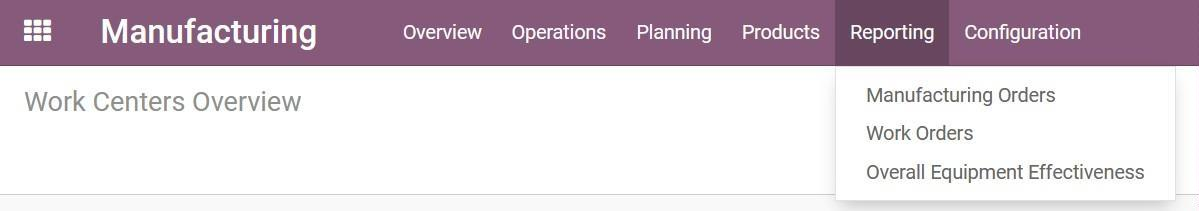
\includegraphics[width=440.48pt,height=77.50001pt]{latexImage_d88162078ea529d5c1cd8a8082002f9a.png}}
\end{picture}
\newpage
\begin{tikzpicture}[overlay]\path(0pt,0pt);\end{tikzpicture}
\begin{picture}(-5,0)(2.5,0)
\put(500.14,-731.336){\fontsize{12}{1}\usefont{T1}{cmr}{m}{n}\selectfont\color{color_29791}4 }
\put(60.024,-730.616){\fontsize{9.96}{1}\usefont{T1}{cmr}{m}{n}\selectfont\color{color_29791} }
\put(88.1,-72.21997){\fontsize{12}{1}\usefont{T1}{cmr}{m}{n}\selectfont\color{color_29791}除了使用此路徑之外,產品項的UI還具有一個選項卡,該選項卡指向與產品相關}
\put(70.104,-87.82001){\fontsize{12}{1}\usefont{T1}{cmr}{m}{n}\selectfont\color{color_29791}的每月產量比較(圖 }
\put(70.104,-103.54){\fontsize{12}{1}\usefont{T1}{cmr}{m}{n}\selectfont\color{color_29791}72)。如果Odoo的試用版有一個多月的時間,那會更令人印象深刻。 }
\put(60.024,-121.66){\fontsize{14.52}{1}\usefont{T1}{cmr}{m}{n}\selectfont\color{color_29791} }
\put(60.024,-332.05){\fontsize{11.52}{1}\usefont{T1}{cmr}{m}{n}\selectfont\color{color_29791} }
\put(208.61,-345.97){\fontsize{12}{1}\usefont{T1}{cmr}{m}{n}\selectfont\color{color_29791}圖 72 產品項中關於 MO 的總量 }
\put(60.024,-367.33){\fontsize{18}{1}\usefont{T1}{cmr}{m}{n}\selectfont\color{color_29791} }
\put(132.02,-383.53){\fontsize{12.96}{1}\usefont{T1}{cmr}{m}{n}\selectfont\color{color_29791}1. 查找生產編號有多容易? }
\put(60.024,-399.49){\fontsize{12}{1}\usefont{T1}{cmr}{m}{n}\selectfont\color{color_29791} }
\put(88.1,-413.53){\fontsize{12}{1}\usefont{T1}{cmr}{m}{n}\selectfont\color{color_29791}除了前面提到的方法外,Odoo還提供了一個單位預測圖,記錄了庫存的來龍去脈}
\put(70.104,-429.15){\fontsize{12}{1}\usefont{T1}{cmr}{m}{n}\selectfont\color{color_29791}。這對於估算銷售量和平衡存儲與需求特別有用(圖 }
\put(70.104,-444.75){\fontsize{12}{1}\usefont{T1}{cmr}{m}{n}\selectfont\color{color_29791}73)。這個功能在這項工作中沒有太多提及,因為供求關係與其說是MES功能,不}
\put(70.104,-460.35){\fontsize{12}{1}\usefont{T1}{cmr}{m}{n}\selectfont\color{color_29791}如說是對生產有一個概述是有用的。}
\put(70.05,-320.95){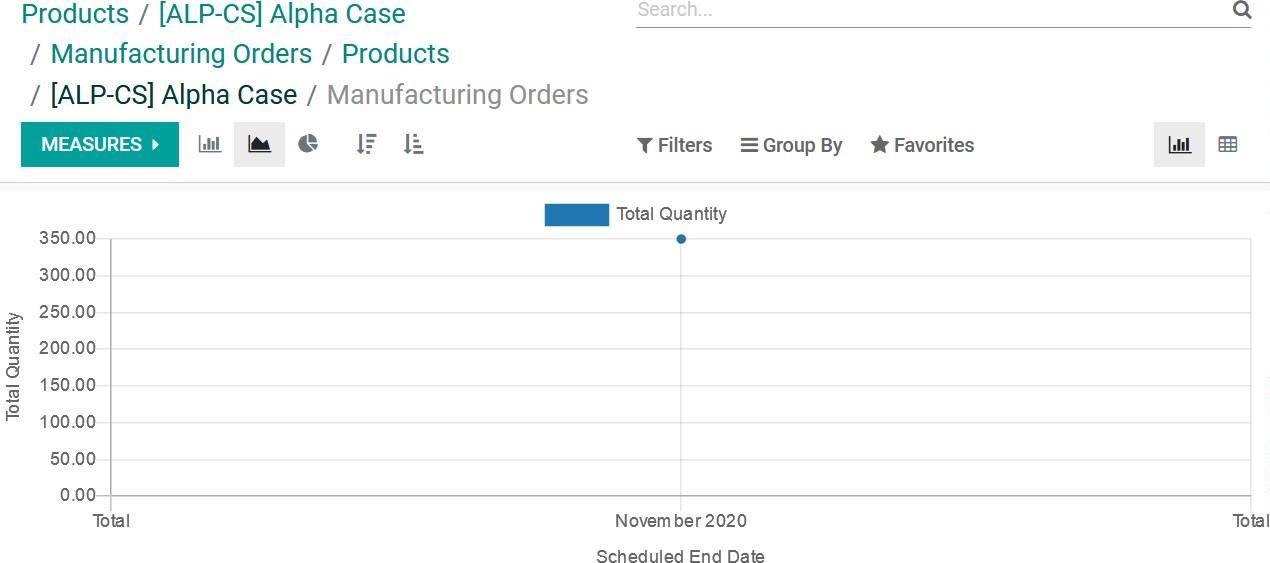
\includegraphics[width=438.22pt,height=194.2pt]{latexImage_c696b639b51d32942de93f78c9eed786.png}}
\end{picture}
\newpage
\begin{tikzpicture}[overlay]\path(0pt,0pt);\end{tikzpicture}
\begin{picture}(-5,0)(2.5,0)
\put(500.14,-731.336){\fontsize{12}{1}\usefont{T1}{cmr}{m}{n}\selectfont\color{color_29791}5 }
\put(60.024,-730.616){\fontsize{9.96}{1}\usefont{T1}{cmr}{m}{n}\selectfont\color{color_29791} }
\put(496.9,-281.65){\fontsize{9.96}{1}\usefont{T1}{cmr}{m}{n}\selectfont\color{color_29791} }
\put(60.024,-290.05){\fontsize{8.52}{1}\usefont{T1}{cmr}{m}{n}\selectfont\color{color_29791} }
\put(241.49,-307.81){\fontsize{12}{1}\usefont{T1}{cmr}{m}{n}\selectfont\color{color_29791}圖73 單位預測概覽 }
\put(60.024,-324.13){\fontsize{12.96}{1}\usefont{T1}{cmr}{m}{n}\selectfont\color{color_29791} }
\put(60.024,-342.97){\fontsize{17.04}{1}\usefont{T1}{cmr}{m}{n}\selectfont\color{color_29791} }
\put(132.02,-359.17){\fontsize{12.96}{1}\usefont{T1}{cmr}{m}{n}\selectfont\color{color_29791}2. Odoo如何生成性能數據? }
\put(60.024,-375.13){\fontsize{12}{1}\usefont{T1}{cmr}{m}{n}\selectfont\color{color_29791} }
\put(88.1,-389.17){\fontsize{12}{1}\usefont{T1}{cmr}{m}{n}\selectfont\color{color_29791}敏銳的讀者會注意到,到目前為止提到的所有數據都是從執行操作完成的時間、}
\put(70.104,-404.77){\fontsize{12}{1}\usefont{T1}{cmr}{m}{n}\selectfont\color{color_29791}與MO和使用的工作中心的相關數量得出的。即便如此,可以繪製多少信息還是令人}
\put(70.104,-420.39){\fontsize{12}{1}\usefont{T1}{cmr}{m}{n}\selectfont\color{color_29791}印象深刻,特別是考慮到它都是自動生成的。 }
\put(60.024,-436.83){\fontsize{12.96}{1}\usefont{T1}{cmr}{m}{n}\selectfont\color{color_29791} }
\put(60.024,-455.67){\fontsize{17.04}{1}\usefont{T1}{cmr}{m}{n}\selectfont\color{color_29791} }
\put(106.1,-471.75){\fontsize{12.96}{1}\usefont{T1}{cmr}{m}{n}\selectfont\color{color_29791}3. 軟體如何呈現升級導致的性能變化? }
\put(60.024,-487.59){\fontsize{12}{1}\usefont{T1}{cmr}{m}{n}\selectfont\color{color_29791} }
\put(88.1,-501.63){\fontsize{12}{1}\usefont{T1}{cmr}{m}{n}\selectfont\color{color_29791}為了識別更改,用戶必須識別更改后的MO,並在此基礎上查看差異。理想情況}
\put(70.104,-517.23){\fontsize{12}{1}\usefont{T1}{cmr}{m}{n}\selectfont\color{color_29791}下,如果圖形信息顯示產品的修訂版,那就太好了,但這在}
\put(84.65,-281.65){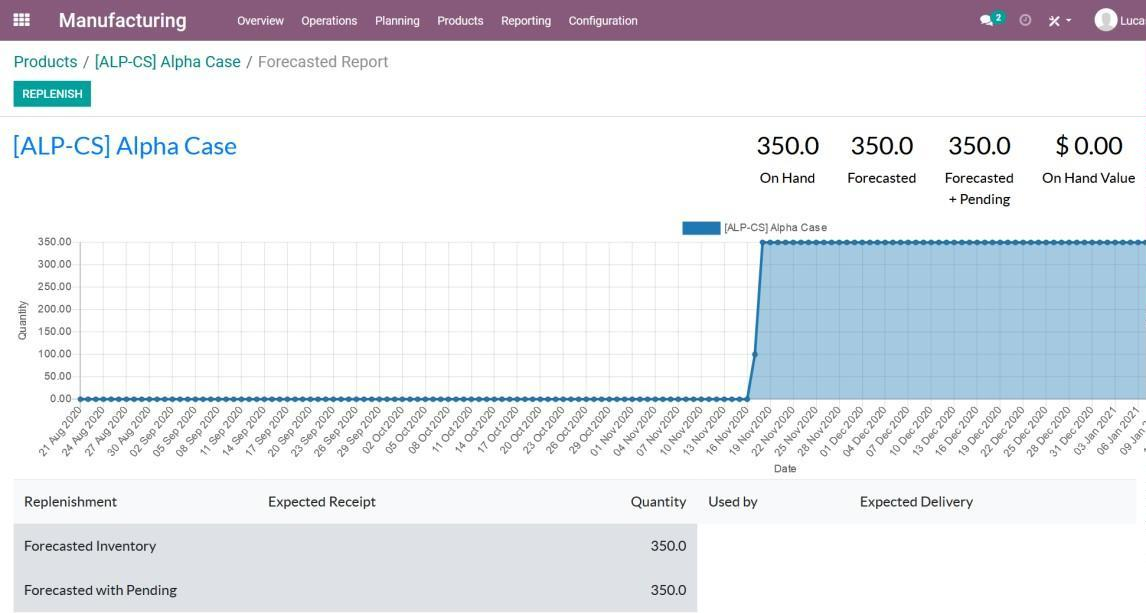
\includegraphics[width=412.18pt,height=220.65pt]{latexImage_98a755ef1b1639e6e7a1d157df567ba2.png}}
\end{picture}
\newpage
\begin{tikzpicture}[overlay]\path(0pt,0pt);\end{tikzpicture}
\begin{picture}(-5,0)(2.5,0)
\put(500.14,-731.336){\fontsize{12}{1}\usefont{T1}{cmr}{m}{n}\selectfont\color{color_29791}6 }
\put(60.024,-730.616){\fontsize{9.96}{1}\usefont{T1}{cmr}{m}{n}\selectfont\color{color_29791} }
\put(275.09,-76.06){\fontsize{15.96}{1}\usefont{T1}{cmr}{m}{n}\selectfont\color{color_29791}結論 }
\put(60.024,-97.53998){\fontsize{17.04}{1}\usefont{T1}{cmr}{m}{n}\selectfont\color{color_29791} }
\put(88.1,-124.9){\fontsize{12}{1}\usefont{T1}{cmr}{m}{n}\selectfont\color{color_29791}在第 2 章中,我引用了一張圖表,該圖表代表了 PLM }
\put(70.104,-140.5){\fontsize{12}{1}\usefont{T1}{cmr}{m}{n}\selectfont\color{color_29791}與其他系統集成的理論理想(圖 }
\put(70.104,-156.1){\fontsize{12}{1}\usefont{T1}{cmr}{m}{n}\selectfont\color{color_29791}74)。在該圖中,讀者可以注意到,理想情況下,PLM將是系統的中心,並附加其}
\put(70.104,-171.7){\fontsize{12}{1}\usefont{T1}{cmr}{m}{n}\selectfont\color{color_29791}他系統(包括ERP)。與上述圖表不同的是,Odoo軟體以ERP為中心,並附加了其}
\put(70.104,-187.3){\fontsize{12}{1}\usefont{T1}{cmr}{m}{n}\selectfont\color{color_29791}他系統。這項工作表明,將Odoo用於PLM和MES當然是可能的,但它也表明PLM和}
\put(70.104,-202.9){\fontsize{12}{1}\usefont{T1}{cmr}{m}{n}\selectfont\color{color_29791}MES的實現存在一些弱點。 }
\put(60.024,-216.46){\fontsize{9.96}{1}\usefont{T1}{cmr}{m}{n}\selectfont\color{color_29791} }
\put(60.024,-225.82){\fontsize{7.56}{1}\usefont{T1}{cmr}{m}{n}\selectfont\color{color_29791} }
\put(60.024,-371.29){\fontsize{12.48}{1}\usefont{T1}{cmr}{m}{n}\selectfont\color{color_29791} }
\put(74.304,-385.45){\fontsize{12}{1}\usefont{T1}{cmr}{m}{n}\selectfont\color{color_29791}圖 74 左邊是 Saaksvuori, A. 和 Immonen, A. (2008) 理論上的改編圖,右邊是 }
\put(209.45,-401.05){\fontsize{12}{1}\usefont{T1}{cmr}{m}{n}\selectfont\color{color_29791}Odoo 對系統如何交互的看法。 }
\put(60.024,-416.41){\fontsize{12}{1}\usefont{T1}{cmr}{m}{n}\selectfont\color{color_29791} }
\put(88.1,-430.47){\fontsize{12}{1}\usefont{T1}{cmr}{m}{n}\selectfont\color{color_29791}缺乏對操作專案、工作中心或設備等檔上傳的支援是一個令人擔憂的問題,特別}
\put(70.104,-446.07){\fontsize{12}{1}\usefont{T1}{cmr}{m}{n}\selectfont\color{color_29791}是考慮到 3D 列印或 CNC,因為訪問 CAD }
\put(70.104,-461.79){\fontsize{12}{1}\usefont{T1}{cmr}{m}{n}\selectfont\color{color_29791}檔對操作員很有説明。此外,當公司自行開發和生產所述工具時,產品和工具的各}
\put(70.104,-477.39){\fontsize{12}{1}\usefont{T1}{cmr}{m}{n}\selectfont\color{color_29791}個方面之間存在差距(在類比中開發模具時也會出現類似的情況)。 }
\put(60.024,-492.75){\fontsize{11.52}{1}\usefont{T1}{cmr}{m}{n}\selectfont\color{color_29791} }
\put(70.104,-506.67){\fontsize{12}{1}\usefont{T1}{cmr}{m}{n}\selectfont\color{color_29791}此外,儘管MES提供了有關其數據集的詳細圖形表示,但它僅限於從執行操作完成}
\put(70.104,-522.27){\fontsize{12}{1}\usefont{T1}{cmr}{m}{n}\selectfont\color{color_29791}時間得出的數據。例如,如果有關品質控制的圖形表示也很容易獲得,那將是非常}
\put(70.104,-537.87){\fontsize{12}{1}\usefont{T1}{cmr}{m}{n}\selectfont\color{color_29791}有價值的。 }
\put(60.024,-553.23){\fontsize{12}{1}\usefont{T1}{cmr}{m}{n}\selectfont\color{color_29791} }
\put(88.1,-567.27){\fontsize{12}{1}\usefont{T1}{cmr}{m}{n}\selectfont\color{color_29791}綜上所述,將ECO應用於Odoo中的BOM是一個值得稱讚的過程。ECO }
\put(70.104,-582.87){\fontsize{12}{1}\usefont{T1}{cmr}{m}{n}\selectfont\color{color_29791}會保留資訊,直到準備好應用,然後在負責人員驗證 ECO 後自動更新 }
\put(70.104,-598.5){\fontsize{12}{1}\usefont{T1}{cmr}{m}{n}\selectfont\color{color_29791}BOM。它現在看起來可能並不那麼重要,因為這個模擬處理的是非常簡單的產品,}
\put(70.104,-614.1){\fontsize{12}{1}\usefont{T1}{cmr}{m}{n}\selectfont\color{color_29791}但隨著複雜性的增加,它變得越來越重要。例如,如果沒有這樣的系統,一輛擁有}
\put(70.104,-629.82){\fontsize{12}{1}\usefont{T1}{cmr}{m}{n}\selectfont\color{color_29791}數千個零件和數百個嵌套 BOM 的汽車將被視為控制和跟蹤變化的噩夢。 }
\put(60.024,-645.18){\fontsize{12}{1}\usefont{T1}{cmr}{m}{n}\selectfont\color{color_29791} }
\put(88.1,-659.22){\fontsize{12}{1}\usefont{T1}{cmr}{m}{n}\selectfont\color{color_29791}該軟體對於PLM或MES的實施並不完美,但在可用性和與其他系統的集成方面確}
\put(70.104,-674.82){\fontsize{12}{1}\usefont{T1}{cmr}{m}{n}\selectfont\color{color_29791}實具有價值。功能就在那裡}
\put(73.15,-359.5){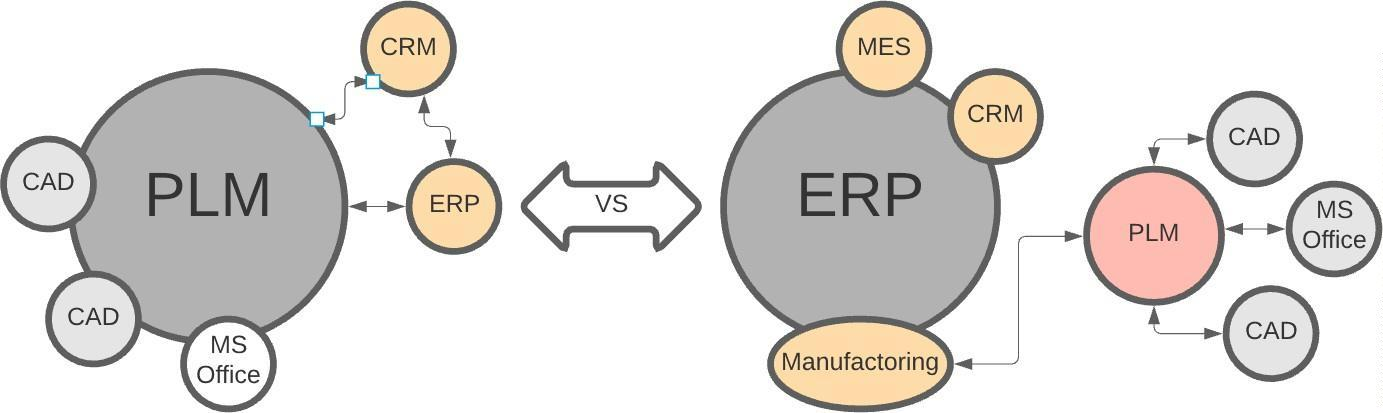
\includegraphics[width=435.49pt,height=130.05pt]{latexImage_babb0ad88ecaa8927aa6f8b4d8ef7c02.png}}
\end{picture}
\newpage
\begin{tikzpicture}[overlay]\path(0pt,0pt);\end{tikzpicture}
\begin{picture}(-5,0)(2.5,0)
\put(500.14,-731.336){\fontsize{12}{1}\usefont{T1}{cmr}{m}{n}\selectfont\color{color_29791}7 }
\put(60.024,-730.616){\fontsize{9.96}{1}\usefont{T1}{cmr}{m}{n}\selectfont\color{color_29791} }
\put(70.104,-72.21997){\fontsize{12}{1}\usefont{T1}{cmr}{m}{n}\selectfont\color{color_29791}特別是在產品和流程方面,該軟體與其自然的ERP功能進行了非常有趣的集成。所有}
\put(70.104,-87.82001){\fontsize{12}{1}\usefont{T1}{cmr}{m}{n}\selectfont\color{color_29791}這些都構成了一個更適合的系統: }
\put(60.024,-103.3){\fontsize{12}{1}\usefont{T1}{cmr}{m}{n}\selectfont\color{color_29791} }
\put(114.02,-121.3){\fontsize{12}{1}\usefont{T1}{cmr}{m}{n}\selectfont\color{color_29791}1. 可以在較小規模中使用 PLM 和 MES 的小型企業。 }
\put(70.104,-132.94){\fontsize{12}{1}\usefont{T1}{cmr}{m}{n}\selectfont\color{color_29791}2. 利用軟體的多合一性質處理較少的製造和更多的組裝或分銷的公司。 }
\put(60.024,-148.3){\fontsize{12}{1}\usefont{T1}{cmr}{m}{n}\selectfont\color{color_29791} }
\put(88.1,-162.34){\fontsize{12}{1}\usefont{T1}{cmr}{m}{n}\selectfont\color{color_29791}值得一提的是,Odoo的局限性不在於產品本身的複雜性,而在於圍繞其開發的操}
\put(70.104,-177.94){\fontsize{12}{1}\usefont{T1}{cmr}{m}{n}\selectfont\color{color_29791}作的複雜性。考慮到所有因素,如果大型複雜裝配僅包含簡單的製造操作或由供應}
\put(70.104,-193.54){\fontsize{12}{1}\usefont{T1}{cmr}{m}{n}\selectfont\color{color_29791}商完成更複雜的工程任務,則可以對其進行跟蹤。也就是說,您可以在Odoo中輕鬆}
\put(70.104,-209.14){\fontsize{12}{1}\usefont{T1}{cmr}{m}{n}\selectfont\color{color_29791}跟蹤摩托車的組裝,但PLM功能還不夠完善,無法跟蹤其動力總成的完整演變/發展}
\put(70.104,-224.74){\fontsize{12}{1}\usefont{T1}{cmr}{m}{n}\selectfont\color{color_29791}。這樣做當然是可能的,但工程團隊需要花費太多的時間和精力,僅僅為了擁有具}
\put(70.104,-240.46){\fontsize{12}{1}\usefont{T1}{cmr}{m}{n}\selectfont\color{color_29791}有ERP功能的多合一解決方案而被認為是值得的。 }
\end{picture}
\newpage
\begin{tikzpicture}[overlay]\path(0pt,0pt);\end{tikzpicture}
\begin{picture}(-5,0)(2.5,0)
\put(500.14,-731.336){\fontsize{12}{1}\usefont{T1}{cmr}{m}{n}\selectfont\color{color_29791}8 }
\put(60.024,-730.616){\fontsize{9.96}{1}\usefont{T1}{cmr}{m}{n}\selectfont\color{color_29791} }
\put(275.09,-76.06){\fontsize{15.96}{1}\usefont{T1}{cmr}{m}{n}\selectfont\color{color_29791}書目 }
\put(60.024,-97.53998){\fontsize{17.04}{1}\usefont{T1}{cmr}{m}{n}\selectfont\color{color_29791} }
\put(60.024,-117.7){\fontsize{17.52}{1}\usefont{T1}{cmr}{m}{n}\selectfont\color{color_29791} }
\put(84.264,-132.94){\fontsize{12}{1}\usefont{T1}{cmr}{m}{n}\selectfont\color{color_29791}Ben Khedher, A., Henry, S., Bouras, A. }
\put(70.104,-150.82){\fontsize{12}{1}\usefont{T1}{cmr}{m}{n}\selectfont\color{color_29791}(2011),“MES與產品生命週期管理之間的集成”。IEEE新興技術與工廠自動化國}
\put(70.104,-168.82){\fontsize{12}{1}\usefont{T1}{cmr}{m}{n}\selectfont\color{color_29791}際會議(ETFA 2011),法國圖盧茲。 }
\put(60.024,-185.14){\fontsize{9.96}{1}\usefont{T1}{cmr}{m}{n}\selectfont\color{color_29791} }
\put(84.264,-198.82){\fontsize{12}{1}\usefont{T1}{cmr}{m}{n}\selectfont\color{color_29791}布朗內爾斯。  可在 <HTTPs://www.brownells.com/rifle-}
\put(70.104,-216.7){\fontsize{12}{1}\usefont{T1}{cmr}{m}{n}\selectfont\color{color_29791}parts/receiver- parts/receivers/lower-receivers/ak-47-fixed-stock-receiver-w-trigger-guard-rear-trunnion- prod97339.aspx>。最後訪問時間為 2020 年 8 月 29 日。 }
\put(60.024,-233.14){\fontsize{10.56}{1}\usefont{T1}{cmr}{m}{n}\selectfont\color{color_29791} }
\put(84.264,-246.85){\fontsize{12}{1}\usefont{T1}{cmr}{m}{n}\selectfont\color{color_29791}德安東尼奧,G.;馬切達,L.;紹薩·貝多拉(Sauza Bedolla),J.;Chiabert, P. }
\put(70.104,-264.73){\fontsize{12}{1}\usefont{T1}{cmr}{m}{n}\selectfont\color{color_29791}(2017),“支持工業 4.0 的 PLM-MES 集成”。PLM 2017,IFIP AICT 517,第 129–137 }
\put(70.104,-282.73){\fontsize{12}{1}\usefont{T1}{cmr}{m}{n}\selectfont\color{color_29791}頁,2017 年。 }
\put(60.024,-298.93){\fontsize{9.96}{1}\usefont{T1}{cmr}{m}{n}\selectfont\color{color_29791} }
\put(84.264,-312.61){\fontsize{12}{1}\usefont{T1}{cmr}{m}{n}\selectfont\color{color_29791}德安東尼奧,G.;紹薩·貝多拉(Sauza Bedolla),J.;基亞伯特,P.;Lombardi, F. }
\put(70.104,-330.61){\fontsize{12}{1}\usefont{T1}{cmr}{m}{n}\selectfont\color{color_29791}(2015),“PLM-MES集成支持協作設計”。國際工程設計會議(ICED }
\put(70.104,-348.49){\fontsize{12}{1}\usefont{T1}{cmr}{m}{n}\selectfont\color{color_29791}2015),義大利米蘭。 }
\put(60.024,-364.93){\fontsize{9.96}{1}\usefont{T1}{cmr}{m}{n}\selectfont\color{color_29791} }
\put(84.264,-378.49){\fontsize{12}{1}\usefont{T1}{cmr}{m}{n}\selectfont\color{color_29791}Hanson, K (2019) “當它對 3D }
\put(70.104,-396.37){\fontsize{12}{1}\usefont{T1}{cmr}{m}{n}\selectfont\color{color_29791}列印模具有意義和沒有意義時”。可在:<HTTPs://www.thefabricator.com/additiverep}
\put(70.104,-414.37){\fontsize{12}{1}\usefont{T1}{cmr}{m}{n}\selectfont\color{color_29791}ort/article/additive/plastic-injection-molds- can-be-3d-printed-quickly>。最後訪問時間為 2020 年 11 月 17 日。 }
\put(60.024,-430.71){\fontsize{10.56}{1}\usefont{T1}{cmr}{m}{n}\selectfont\color{color_29791} }
\put(84.264,-444.39){\fontsize{12}{1}\usefont{T1}{cmr}{m}{n}\selectfont\color{color_29791}MEScenter “MES - 製造執行系統”。可在:<http://mescenter.org/en/articles/108-mes-}
\put(70.104,-462.39){\fontsize{12}{1}\usefont{T1}{cmr}{m}{n}\selectfont\color{color_29791}manufacturing-execution-system>.最後訪問時間為 2020 年 10 月 25 日。 }
\put(60.024,-478.59){\fontsize{9.96}{1}\usefont{T1}{cmr}{m}{n}\selectfont\color{color_29791} }
\put(84.264,-492.15){\fontsize{12}{1}\usefont{T1}{cmr}{m}{n}\selectfont\color{color_29791}邁耶,H.;福克斯,F.;Thiel, K. (2009),「製造執行系統 }
\put(70.104,-510.27){\fontsize{12}{1}\usefont{T1}{cmr}{m}{n}\selectfont\color{color_29791}(MES):最佳設計、規劃和部署」。。麥格勞-希爾。 }
\put(60.024,-526.59){\fontsize{9.96}{1}\usefont{T1}{cmr}{m}{n}\selectfont\color{color_29791} }
\put(84.264,-540.15){\fontsize{12}{1}\usefont{T1}{cmr}{m}{n}\selectfont\color{color_29791}Odoo論壇。可在 <https://www.odoo.com/fr\_FR/forum/aide-1/problems-with- v14-}
\put(70.104,-558.15){\fontsize{12}{1}\usefont{T1}{cmr}{m}{n}\selectfont\color{color_29791}manufacturing-and-inventory-177511> 中獲取。最後訪問時間為 2020 年 10 月 31 日。 }
\put(60.024,-574.47){\fontsize{9.96}{1}\usefont{T1}{cmr}{m}{n}\selectfont\color{color_29791} }
\put(84.264,-588.03){\fontsize{12}{1}\usefont{T1}{cmr}{m}{n}\selectfont\color{color_29791}Redwood,B  (2020) “3D 列印 低運行 注塑}
\put(70.104,-606.06){\fontsize{12}{1}\usefont{T1}{cmr}{m}{n}\selectfont\color{color_29791} 模具”。 可在:<HTTPs://www.3dhubs.com/knowledge-base/3d-}
\put(70.104,-623.94){\fontsize{12}{1}\usefont{T1}{cmr}{m}{n}\selectfont\color{color_29791}printing-low-run-injection-molds/\#design>。最後訪問時間為 2020 年 10 月 16 日。 }
\put(60.024,-640.38){\fontsize{9.96}{1}\usefont{T1}{cmr}{m}{n}\selectfont\color{color_29791} }
\put(84.264,-653.94){\fontsize{12}{1}\usefont{T1}{cmr}{m}{n}\selectfont\color{color_29791}Saaksvuori, A. 和 Immonen, A. (2008),“產品生命週期管理”,第 3 }
\put(70.104,-671.94){\fontsize{12}{1}\usefont{T1}{cmr}{m}{n}\selectfont\color{color_29791}版,Springer,柏林。 }
\put(60.024,-688.256){\fontsize{10.56}{1}\usefont{T1}{cmr}{m}{n}\selectfont\color{color_29791} }
\put(84.264,-701.936){\fontsize{12}{1}\usefont{T1}{cmr}{m}{n}\selectfont\color{color_29791}夏普斯兄弟。槍械設計(2020 年)。提供 <https://sharpsbros.com/mb74-5-45-x- }
\end{picture}
\newpage
\begin{tikzpicture}[overlay]\path(0pt,0pt);\end{tikzpicture}
\begin{picture}(-5,0)(2.5,0)
\put(500.14,-731.336){\fontsize{12}{1}\usefont{T1}{cmr}{m}{n}\selectfont\color{color_29791}9 }
\put(60.024,-730.616){\fontsize{9.96}{1}\usefont{T1}{cmr}{m}{n}\selectfont\color{color_29791} }
\put(70.104,-69.44){\fontsize{12}{1}\usefont{T1}{cmr}{m}{n}\selectfont\color{color_29791}39mm/>。最後訪問時間為 2020 年 8 月 29 日。 }
\end{picture}
\newpage
\begin{tikzpicture}[overlay]\path(0pt,0pt);\end{tikzpicture}
\begin{picture}(-5,0)(2.5,0)
\put(500.14,-731.336){\fontsize{12}{1}\usefont{T1}{cmr}{m}{n}\selectfont\color{color_29791}10 }
\put(60.024,-730.616){\fontsize{9.96}{1}\usefont{T1}{cmr}{m}{n}\selectfont\color{color_29791} }
\put(84.264,-72.21997){\fontsize{12}{1}\usefont{T1}{cmr}{m}{n}\selectfont\color{color_29791}Stancioiu, A (2017) “第四次工業革命工業 4.0” s.l.:Academica Brancusi。 }
\put(60.024,-88.65997){\fontsize{9.96}{1}\usefont{T1}{cmr}{m}{n}\selectfont\color{color_29791} }
\put(84.264,-102.22){\fontsize{12}{1}\usefont{T1}{cmr}{m}{n}\selectfont\color{color_29791}Star Rapid (2020) “10 種最佳塑膠注射成型材料”。適用於: }
\put(70.104,-119.98){\fontsize{12}{1}\usefont{T1}{cmr}{m}{n}\selectfont\color{color_29791}<HTTPs://www.starrapid.com/blog/the-ten-most-popular-plastic-injection-}
\put(70.104,-137.98){\fontsize{12}{1}\usefont{T1}{cmr}{m}{n}\selectfont\color{color_29791}molding- materials/>。最後訪問時間為 2020 年 9 月 20 日。 }
\put(60.024,-154.18){\fontsize{9.96}{1}\usefont{T1}{cmr}{m}{n}\selectfont\color{color_29791} }
\put(84.264,-167.74){\fontsize{12}{1}\usefont{T1}{cmr}{m}{n}\selectfont\color{color_29791}Stark, J. (2015),“產品生命週期管理”,第 3 版,Springer,柏林。 }
\put(60.024,-183.34){\fontsize{12}{1}\usefont{T1}{cmr}{m}{n}\selectfont\color{color_29791} }
\put(84.264,-197.38){\fontsize{12}{1}\usefont{T1}{cmr}{m}{n}\selectfont\color{color_29791}蘇達桑,R.;芬維斯,SJ;斯裡拉姆,RD;Wang, F. }
\put(70.104,-215.5){\fontsize{12}{1}\usefont{T1}{cmr}{m}{n}\selectfont\color{color_29791}(2005),“產品資訊建模框架”。《計算機輔助設計》,第 37 卷第 13 期,第 1399-}
\put(70.104,-233.62){\fontsize{12}{1}\usefont{T1}{cmr}{m}{n}\selectfont\color{color_29791}1411 頁。 }
\put(60.024,-249.97){\fontsize{9.96}{1}\usefont{T1}{cmr}{m}{n}\selectfont\color{color_29791} }
\put(84.264,-263.53){\fontsize{12}{1}\usefont{T1}{cmr}{m}{n}\selectfont\color{color_29791}Tripaldi, M (2019) “評估中型企業的 PLM 實施 - Cubogas 案例研究”,Tesi di }
\put(70.104,-281.53){\fontsize{12}{1}\usefont{T1}{cmr}{m}{n}\selectfont\color{color_29791}laurea,都靈理工大學。  適用於: }
\put(70.104,-299.05){\fontsize{12}{1}\usefont{T1}{cmr}{m}{n}\selectfont\color{color_29791}<https://webthesis.biblio.polito.it/13994/>。最後訪問時間為 2020 年 9 月 23 日。 }
\put(60.024,-313.21){\fontsize{12}{1}\usefont{T1}{cmr}{m}{n}\selectfont\color{color_29791} }
\put(84.264,-327.25){\fontsize{12}{1}\usefont{T1}{cmr}{m}{n}\selectfont\color{color_29791}翁布爾,EJ;哈夫特,R.R.;Umble, M. M. }
\put(70.104,-345.25){\fontsize{12}{1}\usefont{T1}{cmr}{m}{n}\selectfont\color{color_29791}(2003),“企業資源規劃:實施程序和關鍵成功因素”。《歐洲運籌學雜誌》,第 }
\put(70.104,-363.13){\fontsize{12}{1}\usefont{T1}{cmr}{m}{n}\selectfont\color{color_29791}146 卷第 2 期,第 241-257 頁。 }
\put(60.024,-379.57){\fontsize{9.96}{1}\usefont{T1}{cmr}{m}{n}\selectfont\color{color_29791} }
\put(84.264,-393.13){\fontsize{12}{1}\usefont{T1}{cmr}{m}{n}\selectfont\color{color_29791}巴斯克斯,V.K.R.;Escribano, J. F (2017) }
\put(70.104,-411.01){\fontsize{12}{1}\usefont{T1}{cmr}{m}{n}\selectfont\color{color_29791}“ERP實施行政機構作為公司前端和電子商務智慧手機應用程式”,加泰羅尼亞理工大}
\put(70.104,-429.03){\fontsize{12}{1}\usefont{T1}{cmr}{m}{n}\selectfont\color{color_29791}學理學碩士論文。 }
\put(60.024,-445.35){\fontsize{10.56}{1}\usefont{T1}{cmr}{m}{n}\selectfont\color{color_29791} }
\put(84.264,-459.03){\fontsize{12}{1}\usefont{T1}{cmr}{m}{n}\selectfont\color{color_29791}沃馬克,J.P.;鐘斯,D.T.;Ross, D. (1990),“改變世界的機器”,第 1 期 }
\put(70.104,-476.67){\fontsize{12}{1}\usefont{T1}{cmr}{m}{n}\selectfont\color{color_29791}Edition, Rawson Associates, 紐約. }
\put(70.104,-494.07){\fontsize{12}{1}\usefont{T1}{cmr}{m}{n}\selectfont\color{color_29791} }
\end{picture}
\end{document}